\chapter{常见可逆隐藏算法介绍}
\label{chap:related_intro}
当今可逆隐藏领域的研究主要以图像为载体,虽然也有针对其他载体的可逆隐藏算法,但是
最成熟的算法仍然集中在灰度图像领域,例如:基于可逆压缩的
算法\cite{fridrich2001invertible,celik2005lossless}、基于直
方图平移\cite{ni2006reversible,lee2006reversiblee,li2013general}、差值
扩展\cite{tian2003reversible,alattar2003reversible,alattar2004reversible,alattar2004reversible}、
预测误差扩展的算法\cite{thodi2007expansion},基于整数变换的算法
\cite{coltuc2007very,chen2010reversible,wang2010efficient,peng2012adaptive},以
及能够较大程度上提升可逆隐藏效果的排序技术
\cite{kamstra2005reversible,sachnev2009reversible}本节将对灰度图像和
彩色图像的常用可逆隐藏算法进行详细的回顾和总结。



\section{灰度图像可逆隐藏算法}
\subsection{可逆压缩}
\begin{itemize}
  \setlength{\parindent}{2em}
  \vspace{-2mm}
  \item \textbf{早期基于可逆压缩算法}
    \vspace{-2mm}
    \par
    早期的可逆隐藏算法主要基于可逆压缩算法,而可逆隐藏的本质也可以归于可逆压缩领
    域。基于可逆压缩的可逆隐藏算法的本质是对载体图像的一个特征集$S$进行可逆压缩,
    利用压缩出的部分空间进行消息嵌入。嵌入的简单实现是将$S$换为其压缩形式$S_c$和
    消息$M$,因此最大的嵌入容量(Embedding Capacity, EC)为$S-S_c$。显然基于可逆
    压缩的算法效果取决于压缩算法和选取的特征集。
    \par
    2001年\cite{fridrich2001invertible},Fridrich提出的可逆隐藏算法通过对有最小
    冗余度的位平面(bit-plane with the minimum redundancy)进行压缩来获得空间。
    在他们的算法中,除非图像噪声很大,否则总是最低位平面被用来压缩和隐藏。同年
    \cite{fridrich2001invertible2},Fridrich针对JPEG图像提出了一种基于可逆隐藏的
    算法。该算法对变换域的每个块的固定位置提出其DCT系数,由于DCT变换的性质,这
    些系数构成一个有偏序列,进而可以利用可逆压缩为消息嵌入提供空间。
    \par
    文献\cite{celik2005lossless}中,Celik提出了一种广义LSB替换的算法,改进了
    Fridrich算法的性能。算法首先将图像分成不相交的小块,将块中每个像素对$L$取模
    后的余数序列进行无损压缩。将消息转换成$L$进制后填充压缩出来的空间,再反变换
    为灰度值。这种算法将消息嵌入到每个像素对$L$取模的余数上,通过采用$L$个码元,
    而不是Fridrich算法的2个,提高了嵌入容量。
    \par
    早期基于可逆隐藏的算法最大的问题在于其嵌入容量过小。考虑一个8比特灰度图像,
    每个像素的取值范围为$[0, 255]$,而在基于可逆压缩的算法中,要将一个8比特整数
    映射到一个二元或者$L$元整数,在映射像集进行嵌入。这样载体中大量的可用嵌入空
    间没有得到利用,实际嵌入率为0.1 bpp(bit per pixel,每比特嵌入容量)左右,限
    制了该算法的发展和应用。\\
  \vspace{-10mm}
  \item \textbf{近期基于可逆压缩算法}
    \vspace{-2mm}
    \par
    如前所述,可逆隐藏本质上可以归于可逆压缩,那么基于信息论,可逆隐藏就可以抽
    象出这样一种问题:对于给定的失真界限,一个特定的载体图像的嵌入容量上界是什
    么?对于这个问题,Kalker和Willems在文献\cite{kalker2002capacity}中给出了解
    答。他们认为可逆隐藏问题可以看成一种特殊的率失真问题,在给定失真界限为
    $\Delta$时,率失真函数,即嵌入率上界为:$\rho_{rev}=maximize\{H(Y)\}-H(X)$,
    其中$X$,$Y$分别表示载体和载密信号,而转移概率矩阵为$P_{Y|X}=(y|x)$,即载体
    信号$x$修改为载密信号$y$的概率,应满足失真界$\sum_{x,y}P_X(x)P_{Y|X}(y|x)
    D(x,y)\le\Delta$,其中$D(x,y)$通常定义为平方失真$(x-y)^2$。
    \par
    根据此理论,学者们提出了一些能够达到理论率失真界限的,基于可逆压缩的可逆隐藏
    算法,而所有这些算法都可以看成是文献\cite{kalker2002capacity}中递归编码构造
    (recursive code construction)的改进。下面通过递归直方图修改(recursive 
    histogram modification, RHM),对算法做简单介绍。
    \par
    RHM首先估计最优转移概率$P_{Y|X}(y|x)$和$P_{X|Y}(x|y)$,然后将载体图像分成不
    相交的块,利用一种熵编码的压缩和解压缩算法,基于最优转移概率,将消息递归地通
    过修改每个块的直方图的方式嵌入到每个块中。以一块为例,设块$\textbf{x}=(x_1,
    \cdots,x_K)$满足概率分布$P_X$,基于转移概率$P_{Y|X}(y|x)$,将$S$比特消息
    $\textbf{m}=(m_1,\cdots,m_S)$解压缩为载密序列$\textbf{y}=(y_1,\cdots,y_K)$并
    用$\textbf{y}$替换$\textbf{x}$。由于$\textbf{x}$与$\textbf{y}$相似,基于转移
    概率$P_{X|Y}(x|y)$将$\textbf{x}$压缩得到$O(x)$。为了将来提取消息后恢复$\textbf
    {x}$,应将$O(x)$同下一段$\textbf{S}$比特消息一起,嵌入到下一个块中。
    \par
    利用这种算法,对于给定的载体和消息,这种算法能够最小化嵌入失真。
\end{itemize}

\subsection{基于扩展的算法}
\begin{itemize}
  \setlength{\parindent}{2em}
  \vspace{-2mm}
  \item \textbf{直方图平移算法}
    \vspace{-2mm}
    \par
    基于直方图平移(Histogram Shifting)的算法首先于2006年由Ni等人提出
    \cite{ni2006reversible}。对于自然图像灰度直方图,几乎总存在没有出现的灰度
    值,而最多的出现频数常常在几千或者几万。这样,设频数最大为$f_{max}$,对应
    灰度为$g_{max}$,频数最小为$f_{min}$,对应灰度为$g_{min}$,不妨设$g_{min}>
    g_{max}$。嵌入算法公式如下:
    \begin{equation}
      \label{eq:histo_shift_embedding}
      I_{i,j}=\left\{ \begin{array}{ll}
        I_{i,j}+m & \textrm{$I_{i,j}=g_{max}$}\\
        I_{i,j}+1 & \textrm{$I_{i,j} \in [g_{max}+1,g_{min}-1]$}\\
        I_{i,j}   & \textrm{otherwise}
      \end{array} \right.
    \end{equation}
    即:顺次扫描图像,将灰度在$[g_{max}+1,g_{min}-1]$范围内的像素值加1,这等价于
    在直方图上将这一范围内的柱右移1个单位,此时频数最小的灰度变为$g_{max}+1$,当
    灰度为$g_{max}$时,这个像素被用来隐藏消息:当消息为0时,保持$g_{max}$不变,
    消息为1时,将$g_{max}$改为$g_{max}+1$。
    \par
    之后,基于直方图平移的算法得到了广泛和深入的研究。其中重要的一个改进来
    自2007年Lee的论文\cite{lee2006reversiblee},文献中Lee提出使用图像预测误差的
    直方图进行直方图平移能得到更好的效果。图\ref{fig:lena_hist_compare}是lena图像
    的预测误差直方图和一般直方图的比较。
    \begin{figure}[!hbt]
    \centering 
    \subfigure[lena图像灰度直方图]{
      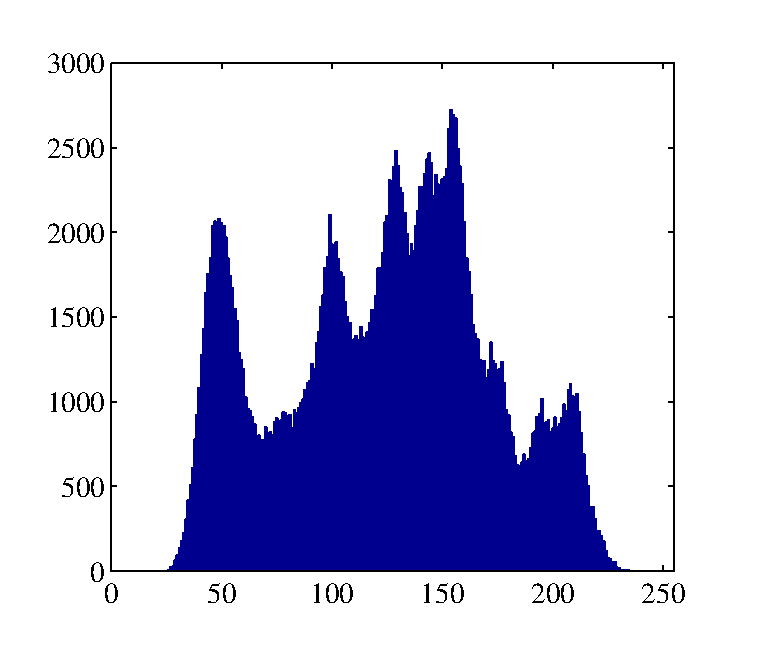
\includegraphics[width=0.4\textwidth]{figures/lena_hist.eps}
      \label{fig:lena_hist}}
    \subfigure[lena图像预测误差直方图]{
      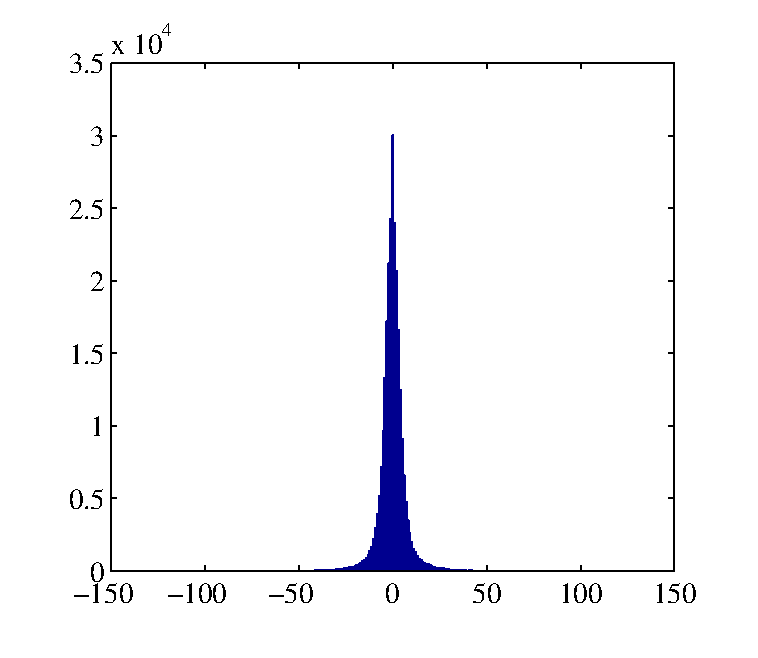
\includegraphics[width=0.4\textwidth]{figures/lena_diffhist.eps}
      \label{fig:lena_diffhist}}
    \caption{lena图像灰度直方图同预测误差直方图的比较}
    \label{fig:lena_hist_compare}
    \end{figure}
    由图中可以看出,同灰度直方图相比,预测误差直方图更加规则,呈Laplace分布,峰
    值位于0点,且比灰度直方图峰值更大。这就意味着使用预测误差直方图将得到更高的
    嵌入容量和更好的图像质量。从这个思路出发,大量的文献对该方法从预测方式到溢
    出问题进行了全面的改进。
  \vspace{-3.5mm}
  \item \textbf{差值扩展算法}
    \vspace{-2mm}
    \par
    这里我们将介绍Tian\cite{tian2003reversible}在2003年提出的差值扩展(Difference
    Expansion, DE)算法。在算法中,载体图像的像素被分为两两不相交的像素对,对每
    个像素对$(x_0, x_1)$,根据整数Haar变换,定义它们的整数均值和差值分别为
    $l=\lfloor (x_0-x_1)/2 \rfloor$和$h=x_1-x_0$。为了嵌入1比特消息$m \in \{0,
    1\}$,差值$h$被扩展为$h'=2h+m$。由整数Haar反变换,载密像素对$(y_0, y_1)$分别为
    $y_0=l-\lfloor h^*/2 \rfloor$和$y_1=l+\lfloor (h^*+1)/2 \rfloor$。通过简单地
    变形,我们得到:
    \begin{equation}
      \label{eq:de_marked_pair}
      \left\{ \begin{array}{l}
        y_0=2x_0-\lceil (x_0+x_1)/2 \rceil\\
        y_1=2x_1-\lceil (x_0+x_1)/2 \rceil+m
      \end{array} \right.
    \end{equation}
    这样,接收端可以通过提取$y_1-y_0$的最低比特位获得消息$m$,并通过$x_0=l^{'}-
    \lfloor h^{'}/2 \rfloor$和$x_1=l^{'}+\lceil h^{'}/2 \rceil$恢复原始像素对
    $(x_0, x_1)$,其中$l^{'}=\lfloor (y_0+y_1)/2 \rfloor$,$h^{'}=\lfloor (y_1-
    y_0)/2 \rfloor$。
    \par
    之后,Alattar\cite{alattar2003reversible,alattar2004reversible,
    alattar2004reversibleg}将差值扩展算法扩展到三像素对、四像素对及$n$像素
    对。在他的扩展中,$n$个像素被变换为一个均值$l$和一个有$n-1$个差值的向量
    $\boldsymbol{\vec{h}}$,对$\boldsymbol{\vec{h}}$的每个元素,都使用二像素对的
    方法进行扩展和消息嵌入。这样,嵌入率从二像素对的0.5 bpp提高到$(n-1)/n$ bpp。
    当选取的$n$合适时,嵌入容量和图像质量之间能得到很好地平衡。
    \par
    差值扩展技术作为可逆信息隐藏的一个基础技术,得到了充分地研究和发展,催生了大
    量新技术的诞生,如基于整数变换的嵌入方法,预测误差扩展算法等。在这些改进中,
    预测误差扩展算法得到了最为广泛的关注。同差值扩展利用两个像素的相关性不同,预
    测误差扩展用到了更大的邻域的相关性,因此可以预期,预测误差将会更加准确,因此
    算法性能将会更好。而预测误差扩展算法也因此成为了现在最为流行的可逆隐藏算法。
    下面将对预测误差扩展算法进行详细介绍。
  \vspace{-3.5mm}
  \item \textbf{预测误差扩展算法}
    \vspace{-2mm}
    \par
    首先先介绍一下预测误差扩展的一般流程:
    \begin{enumerate}[leftmargin=7em,label=\textbf{步骤 \arabic*:}]
      \item{对每个像素进行预测得到预测误差。首先对图像的每个像素$x_{i,j}$,使用一
        个预测器根据其邻域对其进行预测,得到预测值$x_{i,j}^{'}$。然后求预测误差
        $e_{i,j}=x_{i,j}-x_{i,j}^{'}$。}
      \item{通过计算每个预测误差的频数产生预测误差直方图,通常情况下预测误差服从
          Laplace分布,中心在0点或者0点附近。}
      \item{通过扩差和移位,对PEH进行修改。特别的,对预测误差$e_{i,j}$,它被扩展
        或移位为:
      \begin{equation}
        \label{eq:pee_embedding}
        e_{i,j}^{'}=\left\{ \begin{array}{ll}
          2e_{i,j}+m & if~~e_{i,j} \in [-T,T)\\
          e_{i,j}+T  & if~~e_{i,j} \in [T,+\infty)\\
          e_{i,j}-T  & if~~e_{i,j} \in (-\infty,-T)
        \end{array} \right.
      \end{equation}
      其中$T$是与嵌入容量有关的参数,$m$是消息比特。这里位于$[-T,T)$的预测误差被
      用来扩展以嵌入消息;位于$(-\infty,-T)\cup[T,+\infty)$的预测误差被向外移位,
      为扩展的差值提供空间,避免消息提取端的混淆。最后像素被修改为$e_{i,j}^{'}
      +x_{i,j}^{'}$。
      }
    \end{enumerate}
    \vspace{-2mm}
    \par
    由上面公式可以看出,嵌入容量取决于$T$,而像素失真的最大值也为$T$,所以载密图
    像的质量也与$T$有关,因此$T$的选取对算法有着重要的影响。
    \vspace{-2mm}
    \par
    在消息提取端,原始预测误差可以通过对载密图像的预测误差通过
    公式\ref{eq:pee_extraction}操作恢复。原始消息通过取位于$[-2T,2T)$区间内的预
    测误差$e_{i,j}^{'}$的最低比特位恢复。最终,原始图像通过已恢复的预测误差计算
    得出。
    \vspace{-5mm}
    \begin{equation}
      \label{eq:pee_extraction}
      e_{i,j}=\left\{ \begin{array}{ll}
        \lfloor e_{i,j}^{'}/2\rfloor & if~~e_{i,j}^{'} \in [-2T,2T)\\
        e_{i,j}^{'}-T  & if~~e_{i,j}^{'} \in [2T,+\infty)\\
        e_{i,j}^{'}+T  & if~~e_{i,j}^{'} \in (-\infty,-2T)
      \end{array} \right.
    \end{equation}
    \par
    通过利用预测误差直方图,预测误差扩展算法可以隐藏大量的消息信息,同时通过扩差
    和移位,图像失真得到了很好地控制。基于预测误差扩展的算法是当前可逆隐藏领域的
    研究热点和最有效的工具。最近提出的可逆隐藏算法大多数以预测误差扩展为框架,并
    对其中的部分环节进行改进。如使用更好的预测算法\cite{ou2013reversible},双层
    嵌入算法\cite{luo2010reversible},嵌入位置选择\cite{hong2012adaptive},二维
    直方图\cite{ou2013pairwise}等。
\end{itemize}

\subsection{基于整数变换的算法}
整数变换(Integer-to-Interger Transform)同样可以用于可逆隐藏算法中。正如前面所
看到的,差值扩展实质上也是一种整数变换算法。2007年,Coltuc和Chassery
\cite{coltuc2007very}提出了一种叫做可逆对比映射(Reversible Contrast Mapping)的
技术,应用了针对整数对的整数变换。这种算法不需要额外的可逆压缩算法,因此在计算复
杂度上有很高的效率。随后,该算法在2010年由Chen进行了改进\cite{chen2010reversible},
Chen将原始的可逆对比映射扩展到任意长度的整数序列。2010年,Wang
\cite{wang2010efficient}利用整数变换将差值扩展算法进行了推广。他们指出差值扩展算
法的嵌入规则可以被重组为一个整数对的变换,并将这种变换推广到了任意大小的像素块。
近期,通过从另一个视角审视差值扩展,Peng\cite{peng2012adaptive}提出了一种全新的
算法。算法首先根据预计算的失真将图像块分类,针对不同的图像块,使用不同的参数进行
整数变换。通过这种自适应的算法,消息更多地被隐藏在了平滑的图像块中,避免了嵌入噪
声块中造成的大失真,从而保证了较高嵌入容量下较好的图像质量。
\par
简而言之,基于整数变换的算法将两个或更多地像素组成一组,通过整数变换将消息分别嵌
入每一个组中,有较好的效果。但是,整数变换算法的预测算法并不准确,仅仅是使用一组
中像素的均值来预测该组中所有的像素。另外,同预测误差扩展算法相比,基于整数变换的
算法并不能控制图像的最大失真。由此可以确定,基于整数变换的算法仅仅对需要大嵌入容
量,而对图像质量有较少关注的应用中适用。

\subsection{排序技术}
在几乎所有的可逆隐藏算法中,都会使用位置地图(Location Map)来辅助消息提取端进行
消息提取和图像恢复。例如在差值扩展中,某些像素会出现上溢或下溢的问题,即当由于差
值的扩大而使得载密像素对不在$[0,255]$范围内时,这个像素对将不能用来隐藏消息。而为
了将这些像素对同那些载密像素对进行区分,就需要用一个位置地图对这些不能嵌入消息的
像素对进行记录:不能嵌入的像素对在位置地图中被设为1,可嵌入像素对被设为0。对于直
方图平移算法、预测误差扩展等算法都有相同的问题。通过对像素对或者像素进行打分、排
序,根据排序结果按顺序嵌入,最终的位置地图就可以被压缩到可以忽略不计的大小,因此
排序技术是可逆隐藏算法中一项非常重要的技术。
\par
使用排序技术的算法又被称为基于内容自适应的可逆隐藏算法(Content-Adaptive RDH),
最早的算法由Kamstra 和Heijmans 提出\cite{kamstra2005reversible}。文献对Tian的差
值扩展算法进行了改进,根据像素对的局部方差对像素对进行排序,依据排序结果依次对像
素对进行嵌入。注意到在差值扩展算法中,像素对的均值是不变的,只有其差值被修改,因
此像素对均值在嵌入端和提取端保持不变,双方都可以用此来计算局部方差。显然如果局部
方差越小,这个像素对应该在图像的纹理平滑区域,那么像素对的差值应越小,从而可嵌入
消息的可能性越大,位置地图越短。文献的实验结果表明使用排序的算法比原始算法有很大的
\begin{figure}[!h]
\centering 
\subfigure[排序前Airplane预测误差]{
  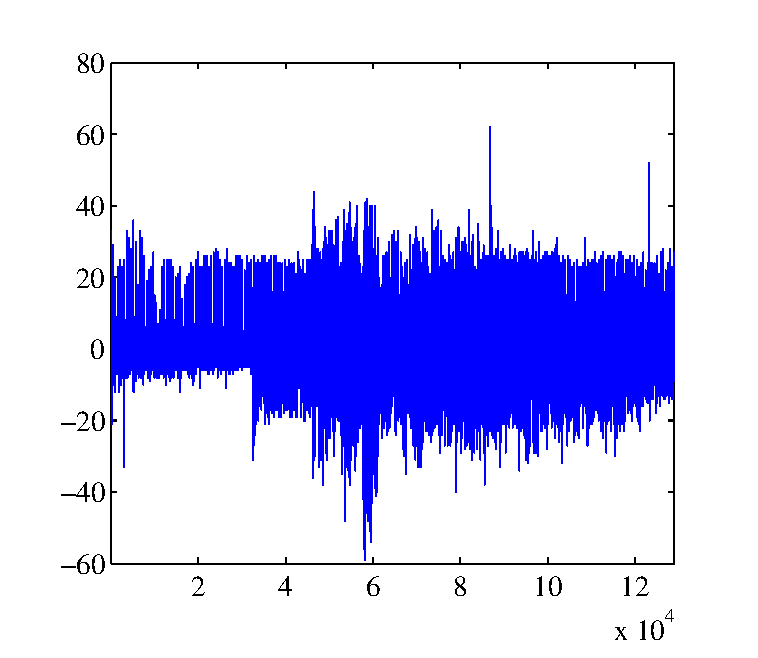
\includegraphics[width=0.4\textwidth]{figures/airplane_original_pe.eps}
  \label{fig:airplane_origin_pe}}
\subfigure[排序后Airplane预测误差]{
  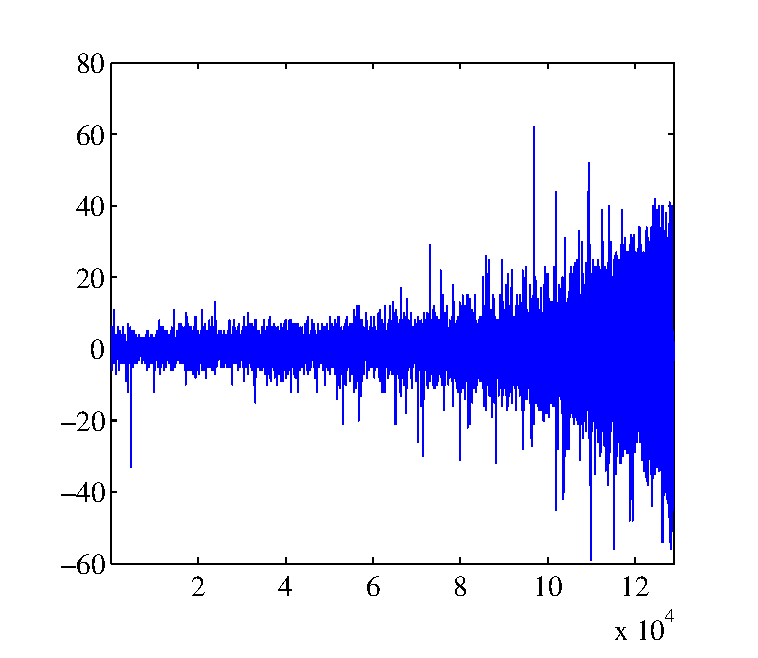
\includegraphics[width=0.4\textwidth]{figures/airplane_sorted_pe.eps}
  \label{fig:airplane_sorted_pe}}
\caption{lena图像灰度直方图同预测误差直方图的比较}
\label{fig:airplane_pe_compare}
\end{figure}
提升。最近的文献也表明\cite{sachnev2009reversible,hong2012adaptive},
将排序技术(或像素选择、嵌入位置选择等)同其他的可逆隐藏算法(如预测误差扩展)结
合,同样能使实验结果获得显著的提升。
\par
如图\ref{fig:airplane_pe_compare}所示,左侧是未排序之前Airplane图像的预测误差,
可以看到,预测误差在0附近波动很大。当利用邻域像素方差进行排序后得到的预测误差如
图\ref{fig:airplane_pe_compare}右侧所示,可以明显的看到,预测误差的绝对值呈现出
由小到大的增长顺序。由于小预测误差优先被用来嵌入,因此载密图像质量可以得到明显提
升。
\par
排序技术的关键是对每个像素或者像素对赋予一个关于图像复杂度的度量,以决定其位于图
像纹理平滑区域还是纹理复杂区域。然后,依据像素纹理复杂程度将纹理平滑的像素或像素
块排在靠前的位置。通过排序使得那些纹理相对平滑的区域被用来嵌入的可能性变大。而由
于纹理越平滑,预测误差就越小,从而用来嵌入时失真也越小。由此可见,排序技术对于改
善可逆信息隐藏的效果有着至关重要的作用。



\section{彩色图像可逆隐藏算法}
基于灰度图像的可逆隐藏算法得到了信息隐藏领域的广泛和深入的研究。但是在现实生活中
,使用最多的还是彩色图像而非灰度图像。但是针对彩色图像的可逆隐藏算法却没有得到深
入的研究。在2013年,Li等人提出了一种基于彩色图像通道相关性的可逆隐藏算法
\cite{li2013reversible}。文献中发现了这样一种彩色图像的通道相关性:一个通道
内的图像边缘方向同另外通道内的图像边缘方向是相同的。图\ref{fig:lena_canny}给出了
Lena图像RGB三个通道Canny算子求得的边缘:
\begin{figure}[!hbt]
\centering 
\subfigure[Canny边缘-R通道]{
  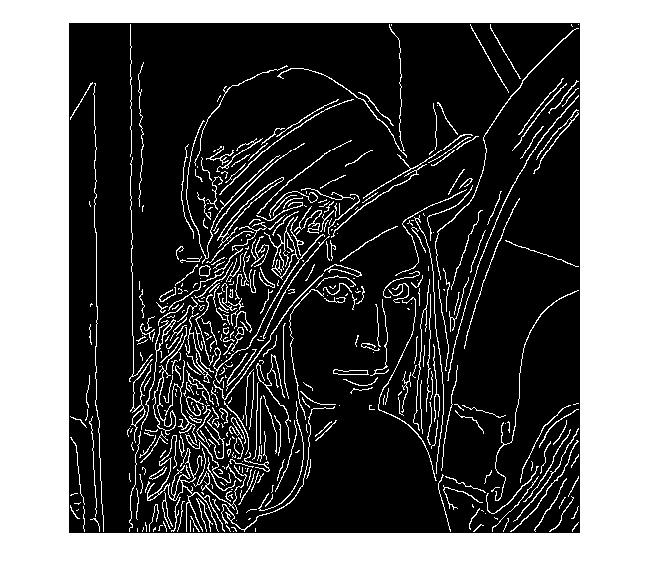
\includegraphics[width=0.3\textwidth]{figures/lena_r_canny.jpg}
  \label{fig:lena_r_canny}}
\subfigure[Canny边缘-G通道]{
  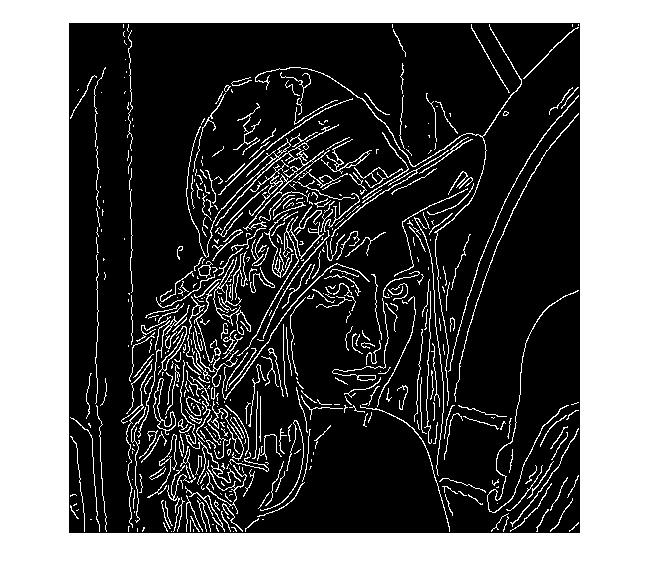
\includegraphics[width=0.3\textwidth]{figures/lena_g_canny.jpg}
  \label{fig:lena_g_canny}}
\subfigure[Canny边缘-B通道]{
  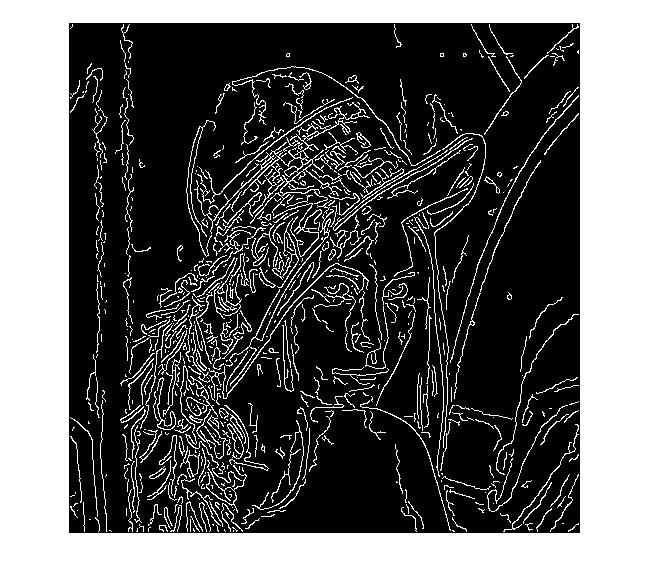
\includegraphics[width=0.3\textwidth]{figures/lena_b_canny.jpg}
  \label{fig:lena_b_canny}}
\caption{Lena图像三个通道边缘信息}
\label{fig:lena_canny}
\end{figure}
从图像中可以看出,在一个通道内的边缘部分,在另一个通道内也基本是边缘部分,同时边
缘方向也基本相同。基于此,文中的预测算法能够较好地对纹理复杂区域的像素进行较好的
预测。
\begin{figure}
  \centering
  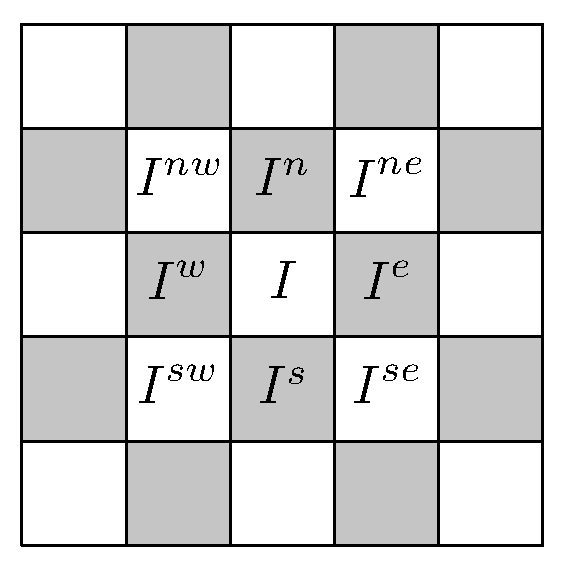
\includegraphics[width=0.3\textwidth]{figures/pixel_neighbourhood.eps}
  \caption{像素$I$的邻域像素}
  \label{fig:pixel_neighbour}
\end{figure}
\par
算法的预测过程如下:设当前通道内的像素为$I_c$,对应的参考通道内的像素为$I_r$。为
了决定当前像素是否在边缘区域,定义两个值。一个表示$I_r$与其邻域内8个像素的距离,
设为$D_m$,像素的8个邻域如图\ref{fig:pixel_neighbour}所示。
\begin{equation}
  D_m=\left|\sum_{k=1}^{8}\lambda_{m}^{k}I_{r}^{k}-I_r\right|
\end{equation}
其中$\lambda_{m}^{k}=1/8$,$I_{m}^{k}(k=1,2,\cdots,8)$表示如图\ref{fig:pixel_neighbour}
所示的8个邻域点。显然当一个像素位于纹理平滑区域时,$D_m$会很小。
\par
另一个值与边缘有关。通过对一个系数向量$\boldsymbol{\lambda_e}$取不同的取值,得到
另一个值$D_e$:
\begin{equation}
  D_e=\left|\sum_{k=1}^{8}\lambda_{e}^{k}I_{r}^{k}-I_r\right|
\end{equation}
$D_e$可以从多个方向的预测误差中选出。文献中使用了四个预测误差:
\begin{equation}
  \begin{array}{ll}
  D_h=\left|\frac{\displaystyle I_r^{w}+I_r^{e}}{\displaystyle 2}-I_r\right| &
  D_v=\left|\frac{\displaystyle I_r^{n}+I_r^{s}}{\displaystyle 2}-I_r\right|\\
  D_d=\left|\frac{\displaystyle I_r^{nw}+I_r^{se}}{\displaystyle 2}-I_r\right| &
  D_{ad}=\left|\frac{\displaystyle I_r^{ne}+I_r^{sw}}{\displaystyle 2}-I_r\right|\\
  \end{array}
\end{equation}
则$D_e=min\{D_h,D_v,D_d,D_{ad}\}$,$\boldsymbol{\lambda_e}$取相应的取值,例如当
$D_e=D_h$时,$\boldsymbol{\lambda_e}=(0,0,0,1/2,1/2,0,0,0)$。
\par
我们知道,在图像的纹理平滑区域,一个像素同它邻域像素的值相似,因此,$D_m$和$D_e$
都应接近于0,它们的差也接近0;另一方面,在图像的纹理复杂区域,一个像素同它边缘方
向上的各个像素相似,而与其他邻域的像素有较大差异,因此$D_m$较大,而$D_e$接近于0,
从而它们的差值也较大。因此,设定临界值$\tau$,当$|D_m-D_e|>\tau$,像素位于纹理复
杂区域,$|D_m-D_e|\le\tau$时,图像位于纹理平滑区域。从而当前通道内的预测值为:
\begin{equation}
  \hat{I}_c=\left\{ \begin{array}{ll}
    \frac{\displaystyle I_c^w+I_c^e+I_c^n+I_c^s}{\displaystyle 4} &
    |D_m-D_e|\le\tau\\
    \sum_{k=1}^{8}\lambda_e^kI_c^k &
    |D_m-D_e|>\tau
  \end{array} \right.
\end{equation}
基于此预测值,获得预测误差直方图,利用预测误差扩展和排序技术,进行可逆隐藏。经试
验分析,该算法同简单地将灰度图像的可逆隐藏算法分别应用到三个通道相比,能得到更高
的嵌入容量,更好的图像质量。
\par
本论文的算法将对该算法进行一定地改进,具体内容将在下一章给出。
